\chapter{Lampiran B. Tangkapan Layar Hasil Pengujian Kinerja}

\begin{figure}[!htb]
	\centering
	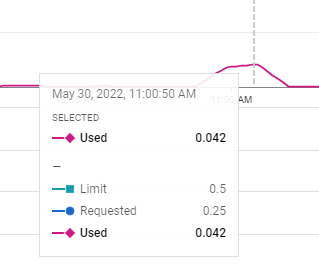
\includegraphics[width=0.5\textwidth]{resources/ch4/resource/1-cpu.png}
	\caption{Penggunaan CPU pada kasus \textbf{SI1}}
	\label{result_cpu_1}
\end{figure}

\begin{figure}[!htb]
	\centering
	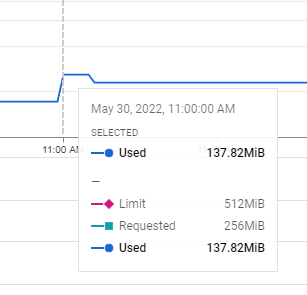
\includegraphics[width=0.5\textwidth]{resources/ch4/resource/1-mem.png}
	\caption{Penggunaan Memory pada kasus \textbf{SI1}}
	\label{result_mem_1}
\end{figure}

\begin{figure}[!htb]
	\centering
	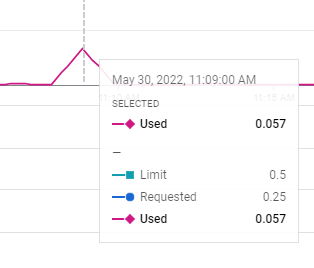
\includegraphics[width=0.5\textwidth]{resources/ch4/resource/2-cpu.png}
	\caption{Penggunaan CPU pada kasus \textbf{SI2}}
	\label{result_cpu_2}
\end{figure}

\begin{figure}[!htb]
	\centering
	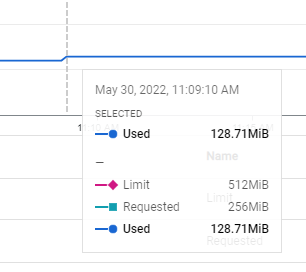
\includegraphics[width=0.5\textwidth]{resources/ch4/resource/2-mem.png}
	\caption{Penggunaan Memory pada kasus \textbf{SI2}}
	\label{result_mem_2}
\end{figure}